\documentclass[deposito, acronym, symbols]{fei}

\usepackage[utf8]{inputenc}
\usepackage{glossaries}
\usepackage{units}
\usepackage{subcaption} 
\usepackage{float}
\usepackage[portuguese]{algorithm2e}
\usepackage{biblatex}
\usepackage{amsmath}
\usepackage{listings}
\usepackage{amsmath}
\lstset{frame=tb,
language=Python,
aboveskip=3mm,
belowskip=3mm,
showstringspaces=false,
columns=flexible,
basicstyle={\small\ttfamily},
numbers=left,
numberstyle=\tiny\color{gray},
keywordstyle=\color{blue},
commentstyle=\color{dkgreen},
stringstyle=\color{mauve},
breaklines=true,
breakatwhitespace=true,
tabsize=4,
frame=shadowbox,
literate= {á}{{\'a}}1 {â}{{\^a}}1 {ã}{{\~a}}1 {é}{{\'e}}1 {ê}{\^e}1 {ç}{\c{c}}1 {í}{\i}1 {ú}{\'u}1 {ó}{{\'o}}1 {ô}{{\^o}}1 {õ}{{\~o}}1 {Á}{{\'A}}1 {É}{{\'E}}1, }
%%
\usepackage{color}
\definecolor{dkgreen}{rgb}{0,0.6,0}
\definecolor{mauve}{rgb}{0.58,0,0.82}

\usepackage{xcolor, multicol,colortbl}
\usepackage[utf8]{inputenc}
\usepackage{chngcntr} %Faz com que o número das notas de rodapé aumente crescentemente
\usepackage{appendix}
\counterwithout{footnote}{chapter} % escrita que precede cada entrada na lista de ilustrações
\renewcommand{\cftfigurepresnum}{Figura }
\setlength{\cftfigurenumwidth}{5.7em}

\usepackage{titling}

%\makeglossaries
%\newacronym[] {achpt} {ACT} {Aparecido ChupeTão}

\newacronym[longplural=Associações Brasileiras de Normas Técnicas]{abnt}{ABNT}{Associação Brasileira de Normas Técnicas}

\newacronym{ibge}{IBGE}{Instituto Brasileiro de Geografia e Estatística}

\newacronym{ashrae}{ASHRAE}{\textit{American Society of Heating, Refrigerating and Air-Conditioning Engineers}}

\newacronym{nbr}{NBR}{Norma Brasileira}

\newacronym{pmv}{PMV}{\textit{Predicted Mean Vote}}
	
\newacronym{ppd}{PPD}{\textit{Predicted Percentage of Dissatisfied}}
		
\newacronym{vgd}{VGD}{Ventilação Geral Diluidor}
		
\newacronym{vgl}{VGL}{Ventilação Local Exaustora}
		
\newacronym{cfd}{CFD}{\textit{Computational Fluid Dynamics}}
		
\newacronym{pcb}{PCB}{\textit{Printed Circuit Board}}
		
\newacronym{sms}{SMS}{\textit{Short Message Service}}
		
%\newglossaryentry{pi}{parent=greek,type=symbols,name={\ensuremath{\pi}},sort=p,description={número irracional que representa [razão entre a circunferência de qualquer círculo e seu diâmetro]}}
		


\title{OTIMIZAÇÃO DA ESTRUTURA OMNIDIRECIONAL DE UM ROBÔ GOLEIRO}
\author{Felipe Estevão Coquito de Mello }
\cidade{São Bernardo do Campo}
\instituicao{Centro Universitário FEI}

\addbibresource{Referencias.bib}
\bibliography{Referencias}
\graphicspath{ {Imagens/} }

\begin{document}
\maketitle

\begin{folhaderosto}
	Relatório Parcial de Iniciação Científica apresentado ao Centro Universitário FEI, como parte dos requisitos do Programa PIBIC-FEI. Orientado pelo Prof. Flavio Tonidandel
\end{folhaderosto}

 \begin{resumo}

O projeto incluiu o desenvolvimento de um novo robô omnidirecional para a categoria \textit{Small-Size} da \textit{RoboCup} de futebol de robôs para a equipe RoboFEI, visando a criação de um robô específico, com a função de ser um goleiro, considerando que atualmente a equipe utiliza o mesmo modelo de robô para todas as funções.

No futebol entre humanos, o goleiro não precisa ter todas as habilidades de um atacante, mas precisa se focar em outras características de sua função, como usar as mãos para defesas e fazer chutes mais longos. Pensando nisso, será estudado um método de redesenho do robô atual para melhor desempenho na defesa do gol e seu impacto nas partidas. Levando em consideração principalmente a cinemática e a dinâmica, será estudada a configuração ideal das rodas e da estrutura do novo robô.


\palavraschave{\textit{RoboCup}. \textit{Small-Size}. Cinemática e Dinâmica. Robô. Omnidirecionais.}

\end{resumo}

\tableofcontents
\listoffigures
\listoftables

\chapter{Introdução}

A categoria \textit{Small Size League} (SSL) é uma das ligas mais antigas da \textit{RoboCup}\footnote[1]{Competição em nível mundial que ocorre anualmente. Com o intuito do estudo e desenvolvimento da Inteligência Artificial (IA) e da Robótica.}, tendo o foco em solucionar o problema da cooperação e controle de robôs inteligentes em ambientes altamente dinâmicos com um sistema híbrido, centralizado/distribuído \cite{about}. Com tal complexidade, é necessário dominar cada aspecto do robô e busca-se a combinação harmônica de diversas áreas do conhecimento para acompanhar o desafio que é estar nesta Liga.

As partidas da categoria ocorrem entre duas equipes no formato 6x6 (\textit{Division B}) ou 11x11 (\textit{Division A}), onde um dos robôs de cada equipe é limitado à linha do gol, sendo este o único jogador permitido a tocar na bola dentro da área sem cometer uma penalidade. Portanto, para cada time é necessário um robô confiável e ágil para essa função de goleiro, sendo este o último recurso para não sofrer algum ponto do adversário.

Para a utilização de um robô na competição, a liga possui regulamentos fixos em relação às especificações que as equipes devem seguir, sendo uma dessas o tamanho máximo dos robôs em campo. É necessário que os jogadores caibam em um cilindro de 180 mm de diâmetro e 150 mm de altura. Existem regras de limite de quanto o robô pode cobrir a área total da bola, entre outras que delimitam o que é um robô da categoria \cite{rules}. Isso cria uma limitação técnica do que é possível incorporar em um novo modelo para a competição. 

\section{Objetivo}

Este estudo tem como objetivo conceber e testar uma nova estrutura omnidirecional de um robô focado na defesa da linha de gol, a qual denominamos de goleiro, na categoria de futebol de robôs SSL, com o intuito de trazer um diferencial competitivo para a equipe RoboFEI e trazer inovações tecnológicas e técnicas para a liga, acelerando cada vez mais sua evolução. 

Serão incorporadas tecnologias modernas para o desenvolvimento dessa estrutura. Na criação do pré-projeto, serão utilizados algoritmos para a obtenção dos ângulos ótimos para a movimentação mais acurada do robô seguindo os caminhos pré-estabelecidos. Além disso, será criado o modelo do robô utilizando o software Autodesk Inventor, para posteriormente iniciar os processos de prototipagem e usinagem do modelo. A ideia é que a metodologia para o desenvolvimento e prototipagem seja de fácil acesso e entendimento, para que caso ocorram eventuais mudanças no regulamento da liga, seja possível estimar e criar um robô que atenda às novas especificações.

\section{Justificativa}

Com o passar dos anos, a competição se tornou cada vez mais competitiva e acirrada. Com isso, as equipes começam a buscar diferenciais entre si na elétrica, mecânica e programação para terem uma vantagem competitiva e conseguirem alcançar a vitória. Porém, mecanicamente, as estruturas apresentam muitas similaridades desde a criação da liga, mudando majoritariamente o sistema frontal de defesa e os materiais empregados na construção do robô, substituindo peças de aço por alumínio, por exemplo \cite{robofei2012}.

A criação de robôs específicos para diferentes funções dentro de campo, similar à escolha de jogadores para cada posição por um técnico analisando suas características físicas, qualidades e defeitos semelhante ao futebol tradicional é algo que nunca foi visto na categoria SSL. A equipe RoboFEI tem a chance de ser pioneira nessa questão, criando uma tendência para a Liga.

A criação de um novo robô abre muitas possibilidades, podendo-se reestruturar várias partes dele como: a estrutura inferior, a configuração das rodas omnidirecionais, o módulo de defesa, a capacidade de chute, entre outros pontos a serem explorados. Baseado em jogos gravados da competição e da equipe RoboFEI, sabe-se que o goleiro tem uma maior movimentação horizontal para realização das defesas na linha do gol. Logo, em uma análise preliminar é possível que a implementação de uma nova configuração levando em conta esse deslocamento horizontal trará o maior benefício imediato para a equipe. 

\chapter{Revisão Bibliográfica}

\section{Sistema Mecânico}

Conjuntos mecânicos são sistemas compostos de máquinas e mecanismos, funcionando em harmonia, podendo ser caracterizados por elementos que interagem entre si para realizar uma função específica, designada pelo projetista e idealizador do projeto. Os elementos podem ser sólidos, fluidos, gasosos ou uma combinação deles. Dentro dos sistemas, os mecanismos são os dispositivos que transformam quaisquer tipos de movimento em um padrão desejado e desenvolvem forças de baixa intensidade e transmitem pouca potência. Já as máquinas são os sistemas que contêm mecanismos que são projetados para fornecer forças significativas e transmitir potência significativa \cite{norton2010cinematica}.Os sistemas mecânicos podem ser classificados em diferentes tipos, de acordo com o seu grau de complexidade, o seu princípio de funcionamento, a sua finalidade ou a sua aplicação.

\subsection{Cinemática e Dinâmica}

A cinemática tem como uma de suas definições o estudo do comportamento das partes de um sistema, independentemente das forças aplicadas para que ocorra a mudança de posição do corpo ao longo do tempo estudado. Portanto, a cinemática descreve como os movimentos se processam, criando assim o projeto do deslocamento desejado dos componentes, buscando estabelecer as formas geométricas das trajetórias dos corpos no espaço e, então, estimar as posições, velocidades e acelerações que esses movimentos irão gerar nos respectivos componentes \cite{norton2010cinematica}. 

Outro aspecto importante no estudo da cinemática é o Referencial, o qual pode ser descrito como a atribuição de três eixos ortogonais entre si que conseguem englobar o objeto de estudo e geram pontos de referência no espaço através do mesmo, possivel observar um exemplo de plano referncial na Figura \ref{fig:planoxyz}. A partir da escolha do referencial do sistema é possível definir os Graus de Liberdade (GDL), que consiste nos números de variáveis independentes que definem o estado do sistema, logo os GDLs representam a quantidade mínima de informação necessária para descrever completamente o estado físico de um sistema. 

\begin{figure}[!htb]
    \centering
    \caption{Plano ortogonal XYZ}
    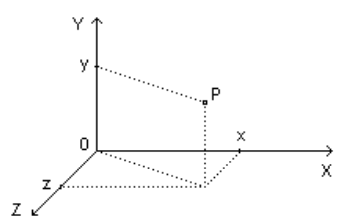
\includegraphics[width=0.5\linewidth]{Imagens/Referencial plano XYZ.png}
    \smallcaption{Fonte: Retirado de \textcite{cinematica}}
    \label{fig:planoxyz}
\end{figure}

A dinâmica tem como objetivo buscar as causas dos movimentos, as forças que agem nos corpos e tem como base a aplicação das três leis de Newton do movimento, sendo assim definida como o estudo do movimento a partir dos seus agentes causadores \cite{cinematica}. A composição do estudo da cinemática e da dinâmica em paralelo é o que norteia a análise de Sistemas Mecânicos, não importando sua complexidade.

\section{Robôs Móveis}

Com a evolução da tecnologia e implementação de circuitos elétricos e algoritmos mais complexos, viu-se a possibilidade de incorporar computadores embarcados em sistemas móveis, integrando sensores e receptores de sinais para a parametrização dos dados, viabilizando a movimentação desses complexos sistemas eletromecânicos.

De acordo com a Japanese Industrial Robot Association (JIRA), robôs podem ser divididos em 6 tipos: \textit{manual handling device}, \textit{fixed sequence robot}, \textit{variable sequence robot}, \textit{playback robot}, \textit{numerical control robot} e \textit{intelligent robot} \cite{nehmzow2012mobile}.

Os robôs moveis autônomos, podem ser parametrizados pelos tipos, 4 a 6 e tem como pricipal diferença a possibilidade de mudar sua localização atraves de movimentação. Sendo essa movimentação possível por alguns tipos de mecanismos como: locomoção por guias no solo ou teto (trilhos), locomoção por combinação de uso de rodas e sistema de locomoção por articulação e apoio (pernas).

\subsection{Robôs Omnidirecionais}

Segundo \textcite{kinematic}, os robôs com rodas Omnidirecionais, também conhecidas como rodas Suiças ou \textit{Mecanum}, têm em seu princípio a capacidade das rodas fornecerem tração na direção normal do motor e paralela ao chão, enquanto a roda pode deslizar sem atrito na direção do eixo do motor,é possivel observar os graus de liberdade descritos na Figura \ref{fig:grausdeliberdade}. 

\begin{figure}[!htb]
    \centering
    \caption{Graus de liberdade de uma roda omnidirecional.}
    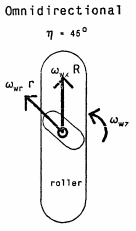
\includegraphics[width=0.3\linewidth]{Graus de liberdade de rodas omnidirecionais.PNG}
    \smallcaption{Fonte: Retirado de \textcite{kinematic}}
    \label{fig:grausdeliberdade}
\end{figure}

Essa movimentação que foge do senso comum é possivel graças a implementação dos \textit{o-rings} com os roletes. Os \textit{o-rings}, são pequenos toroides feitos de polímero ou elastômero que ficam dispostos perpendicularmente em relação à roda principal.Este conjunto forma a parte mais importante para os sistemas omnidirecionais de deslocamento, são responsáveis pela movimentação para qualquer direção no plano XY sem que o robô necesite deslocar seus eixos de lugar \cite{kinematic}. Um exemplo deste conjunto são as rodas que a equipe RoboFEI ultiliza, Figura \ref{fig:rodaExplodida}.

\begin{figure}[!htb]
    \centering
    \caption{Vista explodida da roda.}
    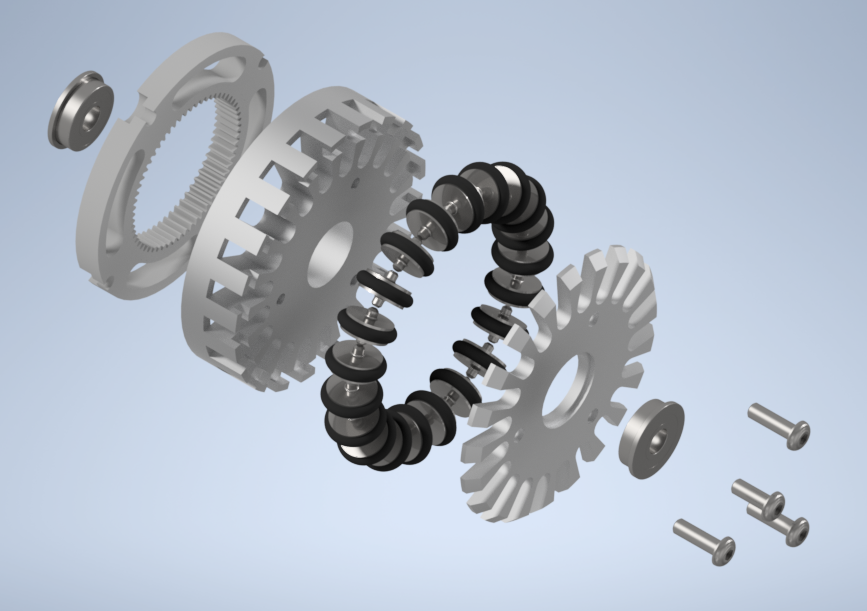
\includegraphics[width=0.6\linewidth]{VistaExplodidaRodaMontada.png}
    \smallcaption{Fonte: Autor}
    \label{fig:rodaExplodida}
\end{figure}

Um aspecto importante para os robôs móveis que utilizam desta forma de roda é que a estabilidade do sistema só é possível com o uso de pelo menos duas rodas omnidirecionais com tração diferencial, porém é aconselhado na literatura a utilização de três ou mais. Segundo \textcite{siegwart2011introduction}, isto se dá pois para alcançar a estabilidade com duas rodas são necessários diâmetros muito grandes de roda e uma grande quantidade de torque nos motores.

Com isso em mente, a estabilidade estática, mais usual, requer um mínimo de três rodas, considerando que o centro de gravidade deve estar contido dentro do triângulo formado pelos pontos de contato das rodas com o solo. A estabilidade pode ser melhorada com a adição de mais rodas, embora uma vez que o número de pontos de contato exceda três, a natureza hiperestática da geometria exigirá algum tipo de suspensão flexível em terrenos irregulares \cite{siegwart2011introduction}. Um exemplo de um robô que opera com sistema de rodas omnidirecionais é o Uranus presente na Figura \ref{fig:Exemploderobo}.

\begin{figure}[!htb]
    \centering
    \caption{Rôbo Uranus}
    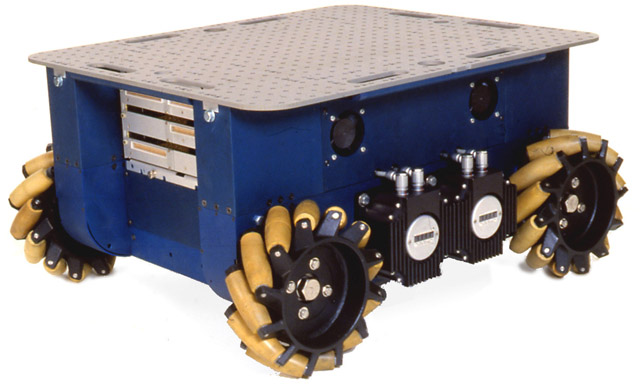
\includegraphics[width=0.45\linewidth]{Imagens/Exemplo de robo.jpg}
    \smallcaption{Fonte: Retirado de \textcite{uranus}}
    \label{fig:Exemploderobo}
\end{figure}

Outro tópico importante quando se trata de robôs com quatro ou três rodas omnidirecionais são os ângulos entre elas. Dependendo da configuração escolhida, há uma influência direta na dinâmica do mesmo. Segundo \textcite{li2019topological} a configuração mais comum para um sistema com 3 rodas \textit{mecanum} é aquela que dispõe as rodas em uma configuração de matriz circular centrípeta, como é possível observar na Figura \ref{fig:configrodas}. As configurações mais comuns para robôs com 4 rodas são a em formato de tanque ou \textit{H-Drive}, que é a configuração usual de automóveis, com os eixos das rodas frontais e traseiras paralelas entre si, e a segunda configuração usual é o \textit{X-Drive}, com os eixos das rodas concorrentes entre si. É possível observar ambos os tipos na Figura \ref{fig:configrodas}.


\begin{figure}[!htb]
        \centering
        \caption{Exemplo de configurações ultilizando 3 e 4 rodas Omnidirecionais}
        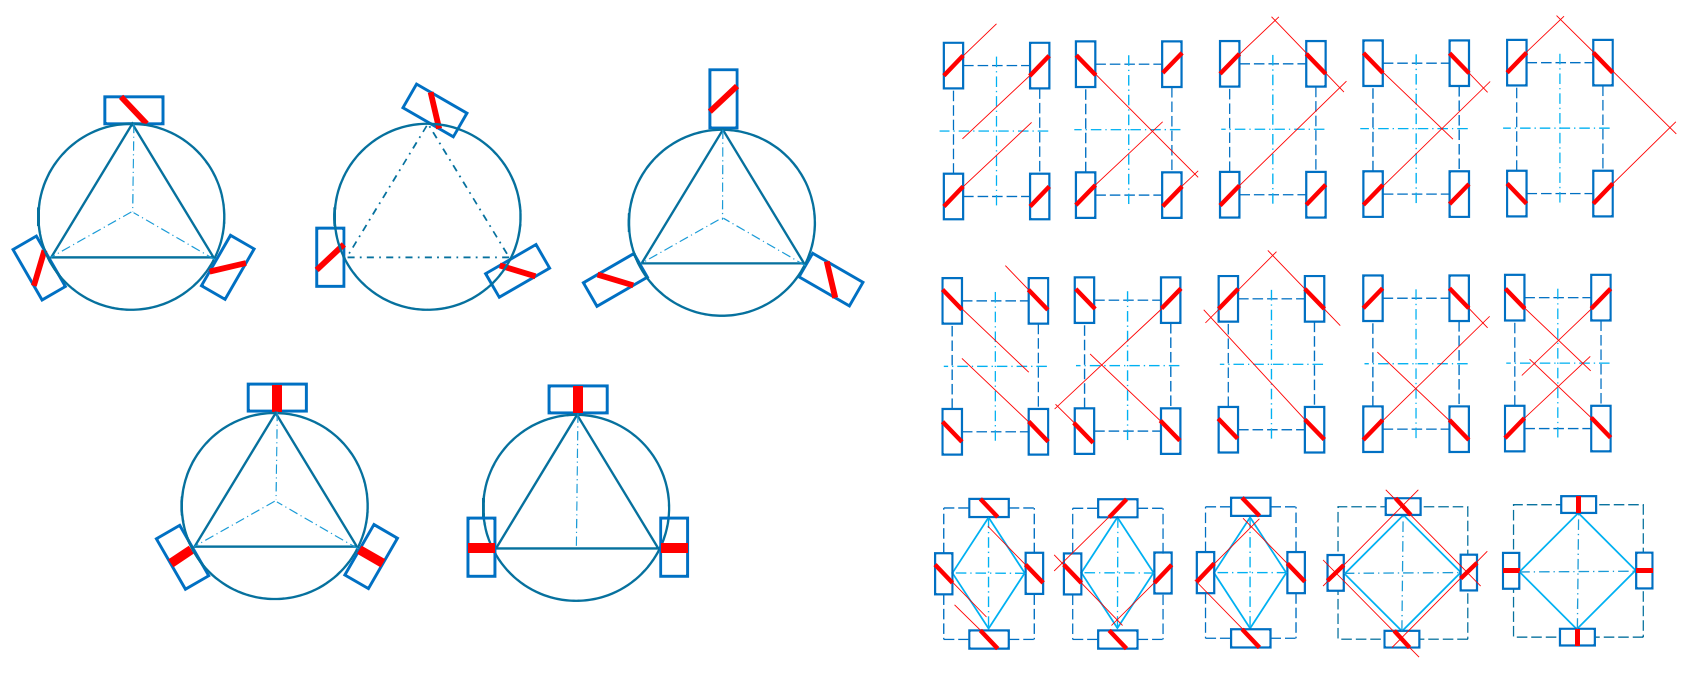
\includegraphics[width=0.9\linewidth]{Imagens/Configurações de rodas.png}
        \smallcaption{Fonte: Retirado de \textcite{li2019topological}}
        \label{fig:configrodas}      
\end{figure}


\chapter{Metodologia}

Será feita a análise da cinemática e dinâmica de um robô omnidirecional com ângulos assimétricos, levando em conta a pesquisa da equipe \textcite{Twente}.

Após a conclusão da pesquisa e das revisões bibliográficas, será desenvolvido um algoritmo para resolver a cinemática direta e inversa do robô estudado. Para validar o funcionamento do código, este será comparado com a movimentação do robô atual da equipe.

Em seguida, a partir do código desenvolvido anteriormente, serão testados individualmente os pares de ângulos das rodas possíveis para o projeto. Para a obtenção dos ângulos otimizados, cada combinação de ângulo será testada individualmente em um percurso estabelecido. Este percurso será concebido com base na movimentação mais tradicional do robô com função de goleiro durante a partida, onde se desloca majoritariamente na horizontal, para realizar as defesas da bola em gol, segundo os vídeos que a equipe RoboFEI possui gravados.

Sucessivamente, após ser concluída essa análise e a partir dos ângulos adquiridos pelo algoritmo, será elaborado o primeiro projeto mecânico estrutural do novo robô utilizando o software CAD, Autodesk Inventor, tendo em vista as necessidades da equipe.

Posteriormente será realizada a impressão 3D do protótipo escolhido, pois ainda se trata do processo de validação da ideia. Em seguida os ajustes finais do protótipo e eventuais novas impressões, o modelo final do novo robô deve ser usinado no CLM (Centro de Laboratórios da Mecânica), para conclusão do projeto e testes comparativos com o atual robô da equipe RoboFEI.


\chapter{Resultados Parciais}

\section{Calculo da Cinemática de Robôs Omidirecionais}

A cinética e dinâmica de robôs omnidirecionais já é estudado à no mínimo três décadas, e existem modelos que definem a movimentação e as variáveis envolvidas. Os estudos de dinâmica dos robôs móveis se baseiam na formulação Newtoniana, utilizado principalmente a segunda lei de Newton, enquanto a formulação da cinética utiliza-se da abordagem da cinemática direta e inversa, que permite encontrar o movimento do robô sabendo a velocidade angular de cada roda, ou o inverso. 

Essa formulação é feita de forma individual por roda considerando seus graus de liberdade, posteriormente são combinadas de forma matricial. A cinemática direta leva em conta os movimentos básicos do objeto, sendo eles: a rotação no próprio eixo ($\omega_r$), deslocamento no eixo X ($V_x$) e deslocamento no eixo Y ($V_y$),que permite encontrar o movimento do robô sabendo a velocidade angular de cada roda. A Figura \ref{fig:cin_clasica} demonstra as velocidades do robô e suas componentes de cada roda o qual é possivel deduzir as equações do movimento.

\begin{figure}[!htb]
    \centering
    \caption{Vista 2D do robô 4 rodas omidirecionais com as velocidades e ângulos}
    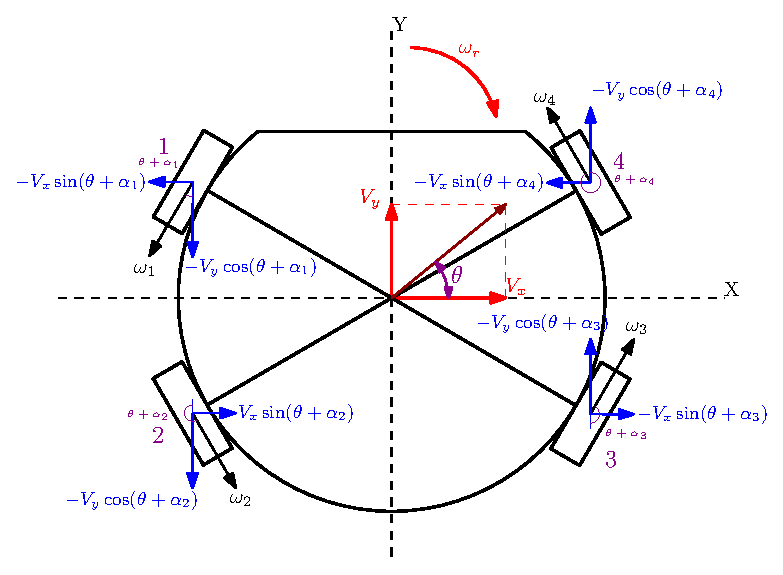
\includegraphics[scale=1]{Imagens/Omni_wheels_clasic.eps}
    \smallcaption{Fonte: Autor} 
    \label{fig:cin_clasica}
\end{figure}

Por conta da evolução dos estudos em robôs omnidirecionais de 4 rodas, na literatura já existem  diversas referências e fórmulas já estabelecidas como a Equação \ref{eq:matrizvelocidade} que é uma adaptação da fórmula proposta por \textcite{rijalusalam2021implementation}.

\begin{equation} \label{eq:matrizvelocidade}
\centering  
\begin{bmatrix}\omega_1\\\omega_2\\\omega_3\\\omega_4\end{bmatrix} = \frac{1}{r} \cdot 
   \begin{bmatrix}-\sin(\theta+\alpha_1)&\cos(\theta+\alpha_1)&R\\-\sin(\theta+\alpha_2)&\cos(\theta+\alpha_2)&R\\-\sin(\theta+\alpha_3)&\cos(\theta+\alpha_3)&R\\-\sin(\theta+\alpha_4)&\cos(\theta+\alpha_4)&R \end{bmatrix}
   \begin{bmatrix}V_x\\V_y\\\omega_r\end{bmatrix}  
\end{equation}

Na equação está descrito: $i\Rightarrow$  1 a 4 o indicie de cada roda, $\omega$ $\Rightarrow$ a velocidade angular do motor; $r$ $\Rightarrow$ o raio da roda;  $\theta$ $\Rightarrow$ o ângulo de movimento do robô, $\alpha$ $\Rightarrow$ o angulo das rodas em relação ao eixo de refenrecia, $R$ $\Rightarrow$ a distância entre as rodas e o centro de massa do robô; $V_x$ $\Rightarrow$ a velocidade do robô na horizontal, $V_y$ $\Rightarrow$ a velocidade do robô na vertical e $\omega_r$ $\Rightarrow$ a rotação do robô.

A partir desta equação é possivel deduzir a matriz para robôs simétricos, com o auxilio de algumas fórmulas de trigonometria básica (\ref{eq:trig}) e considerado a possição inicial da Figura \ref{fig:cin_simetrica}  como $\theta$ = 0 , com essa alterações conseguimos chegar na equação \ref{eq:simetrica}.

\begin{equation} \label{eq:trig}
\centering  
\begin{cases} \sin(a+b)& = \sin(a)\cdot \cos(b) +\sin(b)\cdot \cos(a) \\
              \cos(a+b)& = \cos(a)\cdot \cos(b) -\sin(a)\cdot \sin(b)  \end{cases}
\end{equation}

\begin{figure}[!htb]
    \centering
    \caption{Vista 2D do robô 4 rodas omidirecionais simétrico com as velocidades e ângulos}
    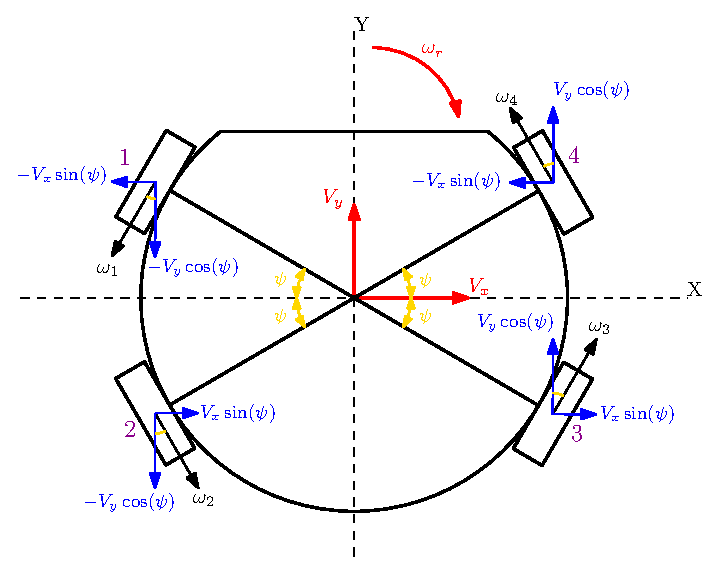
\includegraphics[scale=1]{Imagens/Omini_wheels_simetric.eps}
    \smallcaption{Fonte: Autor} 
    \label{fig:cin_simetrica}
\end{figure}

\begin{equation} \label{eq:simetrica}
\centering  
\begin{bmatrix}\omega_1\\\omega_2\\\omega_3\\\omega_4\end{bmatrix} = \frac{1}{r} \cdot 
   \begin{bmatrix}-\sin(\psi)&\cos(\psi)&R\\
   \sin(\psi)&\cos(\psi)&R\\
   \sin(\psi)&-\cos(\psi)&R\\
   -\sin(\psi)&-\cos(\psi)&R \end{bmatrix}
   \begin{bmatrix}V_x\\V_y\\\omega_r\end{bmatrix}  
\end{equation}
 
\subsection{Calculo da Cinemática de Robôs Omidirecionais Assimétricos}

Os robôs da equipe RoboFEI apresentam atualmente os ângulos $\psi$  todos simétricos entre si a 33º, o que facilita a construção física e o controle dinâmico do robô. Entretanto, isso prejudica uma otimização do robô para uma função específica. 

Com isso em mente e levando em conta o trabalho de \textcite{rojas2005omnidirectional} onde é abordado a ultilização da matriz global de velocidade para robôs omnidirecionais assimétricos, a equipe \textcite{Twente} elaborou apartir deste estudo para a categoria SSL um controle no qual é possível retirar a Equação \ref{eq:cindireta} da matriz de velocidade do robô e a Equação \ref{eq:cininversa} que representa sua pseudoinversa, usando como referencia a Figura \ref{fig:topview}.


\begin{figure}[!htb]
    \centering
    \caption{Vista 2D do robô 4 rodas omidirecionais assimétrico}
    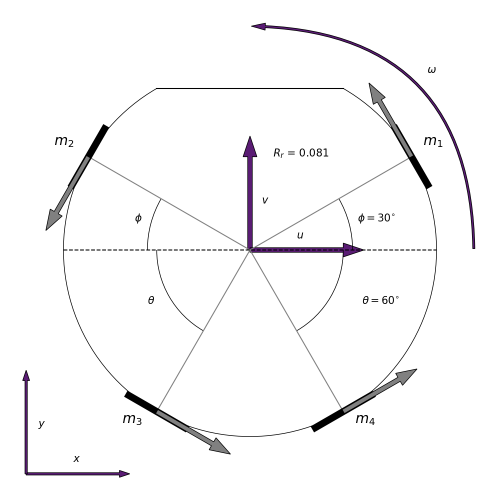
\includegraphics[scale=0.65]{Imagens/topview.png}
    \smallcaption{Fonte: Retirado de \textcite{Twente} } 
    \label{fig:topview}
\end{figure}

\begin{equation} \label{eq:cindireta_1}
\centering  
\begin{bmatrix}\omega_1\\\omega_2\\\omega_3\\\omega_4\end{bmatrix} = \frac{1}{r} \cdot D
   \begin{bmatrix}V_x\\V_y\\\omega_r\end{bmatrix}  
\end{equation}


\begin{equation} \label{eq:cindireta}
\centering  
D = 
\begin{pmatrix}
    -\sin\phi & \cos\phi & R \\ 
    -\sin\phi & -\cos\phi & R \\ 
    \sin\theta & -\cos\theta & R \\ 
    \sin\theta & \cos\theta & R
\end{pmatrix}
\end{equation}


\begin{equation} \label{eq:cininversa}
\centering  
D^\dagger = \frac{1}{2}
\begin{pmatrix}
    -\frac{1}{\sin\theta+\sin\phi} & -\frac{1}{\sin\theta+\sin\phi} & \frac{1}{\sin\theta+\sin\phi} & \frac{1}{\sin\theta+\sin\phi} \\
    \frac{\cos\phi}{\cos^2\theta+\cos^2\phi} & -\frac{\cos\phi}{\cos^2\theta+\cos^2\phi} & -\frac{\cos\theta}{\cos^2\theta+\cos^2\phi} & \frac{\cos\theta}{\cos^2\theta+\cos^2\phi} \\
    \frac{\sin\theta}{\sin\theta+\sin\phi} & \frac{\sin\theta}{\sin\theta+\sin\phi} & \frac{\sin\phi}{\sin\theta+\sin\phi} & \frac{\sin\phi}{\sin\theta+\sin\phi} 
\end{pmatrix}
\end{equation}

\subsubsection{Resultado da otimização dos ângulos}

Considerando trabalhos anteriores da equipe RoboFEI, principalmente os estudos de \textcite{joaorobofei}, onde as rodas da  equipe foram reformuladas para uma versão mais eficiente, é possível voltar a atenção para outra característica importante para a movimentação do robô: os ângulos que cada roda se encontra em relação ao centro geométrico do robô.

Com isso em mente, a otimização dos ângulos das rodas pode ser obtida por diversos métodos. Devido às limitações do projeto, serão selecionados os ângulos de 5º a 35º. Como se trata de uma amostra pequena de combinações de dados, com 900 possibilidades, foi elaborado um código para testar consecutivamente todas essas possibilidades

O código desenvolvido levou em conta os dados fornecidos pela equipe RoboFEI \cite{robofei2023}. Consideramos a utilização, em cada uma das rodas, de um motor Maxon EC 45 flat de 50W em sua tensão nominal de 24 Volts \cite{curvacorrente},  no qual a velocidade nominal é de 5240rpm. No entanto, em medições feitas pela equipe, a roda chega a 1000 rpm em uma relação de transmissão de 1:3, ou seja, uma volta da roda equivale a três voltas do motor. Os motores apresentam uma potência de 3000 rpm no nosso sistema. A partir do estudo\textcite{joaorobofei}, o raio da roda , é de 27 mm e a distância da roda ao centro é de 72 mm. Com esses dados, a equação da cinemática pode ser apresentada como: Equação \ref{eq:robofei} .

\begin{equation} \label{eq:robofei}
\centering  
    \begin{bmatrix} 1000 \cdot \frac{  \bar{\omega_1}}{\left ||\bar{\omega_1} \right ||} \\1000 \cdot \frac{  \bar{\omega_2}}{\left ||\bar{\omega_2} \right ||}\\1000 \cdot \frac{  \bar{\omega_3}}{\left ||\bar{\omega_3} \right ||}\\1000 \cdot \frac{  \bar{\omega_4}}{\left ||\bar{\omega_4} \right ||} \end{bmatrix} = \frac{1}{27 \cdot 10^{-3}}\
\cdot 
    \begin{bmatrix}
    -\sin\alpha & \cos\alpha & 72 \cdot 10^{-3} \\ 
    -\sin\alpha & -\cos\alpha & 72 \cdot 10^{-3} \\ 
    \sin\beta & -\cos\beta & 72 \cdot 10^{-3} \\ 
    \sin\beta & \cos\beta & 72 \cdot 10^{-3}
\end{bmatrix}
   \begin{bmatrix}V_x\\V_y\\\omega_r\end{bmatrix}  
\end{equation}
 
A partir dessa equação da matriz direta e utilizando a matriz inversa, é possível fazer a análise dos ângulos ótimos do robô para a situação desejada.

Com a matriz inversa, é possível fazer o estudo $\bar{\omega_n}$ que corresponde ao sentido que cada roda deve rotacionar para fornecer a movimentação desejada. Foram feitas duas análises distintas: Caso 01; $Vy$ a 1 m/s, $Vx$ a 0.5 m/s e $\omega$ a 0 rad/s e o Caso 02; $Vy$ a 1 m/s e $Vx$ a 0.1 m/s e $\omega$ a 0 rad/s. A partir desses dados, é possível encontrar $\bar{\omega_n}$, que guarda o sentido de rotação de cada roda. Com base no $\bar{\omega_n}$ e o multiplicado pela rotação máxima do motor de 1000 rpm e dividindo pela sua norma, é possível encontrar a rotação máxima de cada roda com seu sentido desejado, sendo isso $\omega_n$ da Equação \ref{eq:cindireta_1}.

A partir do $\omega_n$ de cada roda, é possível analisar qual é o comportamento de cada par de ângulo possível de se combinar, em um código em looping, para ambos os casos. Os resultados de ambas as análises se encontram na Figura \ref{fig:angulo0.5} e Figura \ref{fig:angulo0.1}, tendo seus resultado numérico iguais, onde os ângulos $\alpha$ e $\beta$ devem ser iguais a 22º, como o melhor ângulo para o projeto.

\begin{figure}[!htb]
    \centering
    \caption{Representação gráfica da otimização - Caso 01}
    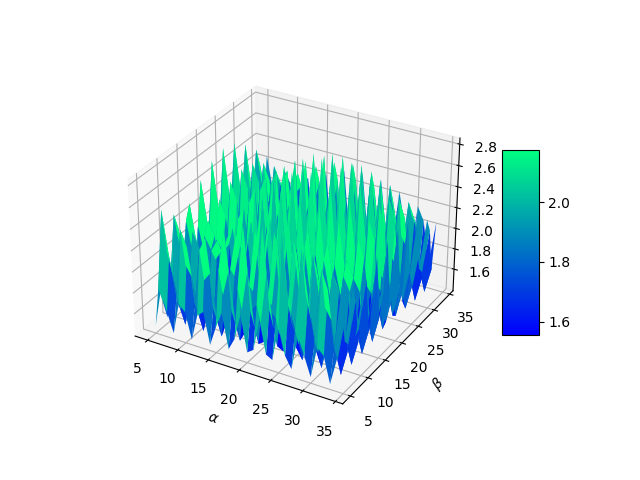
\includegraphics[scale=0.8]{Imagens/Figure_0_5_Vy.png}
    \smallcaption{Fonte: Autor } 
    \label{fig:angulo0.5}
\end{figure}

\begin{figure}[!htb]
    \centering
    \caption{Representação gráfica da otimização - Caso 02}
    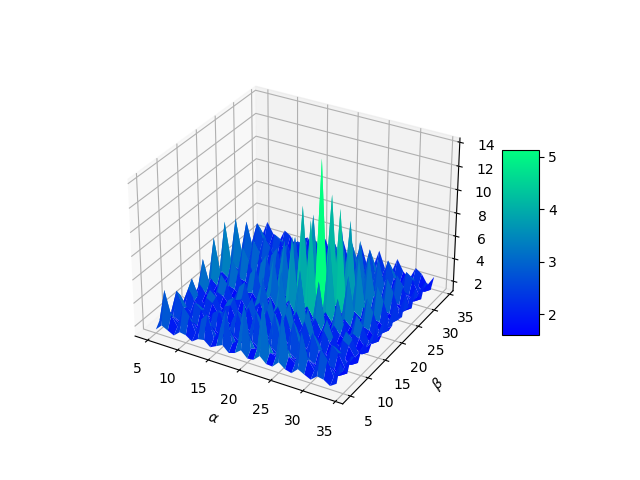
\includegraphics[scale=0.8]{Imagens/Figure_0_1_Vy.png}
    \smallcaption{Fonte: Autor } 
    \label{fig:angulo0.1}
\end{figure}

\chapter{Cronograma}

\definecolor{grey}{rgb}{0.6, 0.6, 0.6}
\newcommand{\X}{\cellcolor{grey}}
\newcommand{\Y}{\cellcolor{blue}}
\begin{table}[!htb]
  \centering
    \caption{Cronograma do desenvolvimento do projeto.}\label{tab:cronograma}
    \scalebox{0.9}
    {\begin{tabular}{>{\raggedright}p{0.30\textwidth}|c|c|c|c|c|c|c|c|c|c|c|c|}
      \cline{2-13}
        Ano 1 & \multicolumn{12}{c|}{Meses} \\ \hline
        Atividades                       &  1 &  2 &  3 &  4 &  5 &  6 &  7 &  8 &  9 & 10 & 11 & 12 \\ \hline \hline
        \small 1) Revisão bibliográfica            & \Y & \Y & \Y &  &  &  &  &  & &  &  &  \\ \hline
        \small 2) Desenvolvimento do Algoritimo   &  &  & \Y & \Y &\Y  &\Y  &  &  & &  &  &    \\ \hline
        \small 3) Projeto em CAD                  &  &  &  &  & &\X  &\X  &    &    &    &    &    \\ \hline
        \small 4) Impressão 3D                    &  &  &  &   &  & &\X   &\X  & & & &  \\ \hline
        \small 5) Usinagem                 &    &    &    &    &    &    &    &  &    & \X &\X   &  \\ \hline
        \small 6) Testes &    &    &    &    &    &    &    &\X    &\X    &    &\X    &    \\ \hline
        \small 7) Análise dos resultados           &    &    &    &    &    &    &    &    &\X    &    &\X    &    \\ \hline
        \small 8) Alteração pós teste &    &    &    &    &  &  &  &    &\X    &    &    &    \\ \hline
        \small 9) Elaboração de relatório parcial &    &    &    &    & \Y & \Y &    &    &    &    &    &    \\ \hline
        \small 9) Elaboração do relatório final  &    &    &    &    &  &  &    &    &    &    & \X   & \X   \\ \hline
    \end{tabular}}
  \smallcaption{Fonte: Autor.}
\end{table}

Na primeira etapa do projeto será realizado um estudo mais detalhado sobre as ideias propostas neste relatório, como a reformulação da estrutura do robô e a configuração das rodas omnidirecionais. 

A segunda etapa é focada na criação e implementação do Algoritimo de Otimização, a fim de obter os ângulos das rodas para o protótipo.

Na terceira etapa será desenvolvido o primeiro protótipo do robô em software CAD. 

A quarta etapa consiste na impressão 3D, e realização dos primeiros testes e análise dos resultados para alterações no protótipo. 

Após finalização dos ajustes e validação no modelo físico impresso, a quinta etapa é a usinagem do robô no CLM e realização dos testes finais, para conclusão do projeto.

Sendo a sexta e última etapa, a coleta dos dados finais e elaboração do relatório final, onde será demonstrado as diferenças entre os dois robôs (atual da equipe e o desenvolvido no projeto), e o impacto que um robô com função específica dentro de jogo pode trazer para a equipe e partidas.

\chapter{Considerações Finais}

Até o momento, os resultados obtidos a partir das pesquisas iniciais são promissores. De modo geral, foi possível obter a equação precisa da cinemática para robôs omnidirecionais assimétricos. Com isso, foi possível implementar o algoritmo da cinemática direta e inversa do modelo. Com o resultado obtido, nas Figuras  \ref{fig:angulo0.5} e \ref{fig:angulo0.1}, de $\alpha$ sendo 22º e $\beta$ sendo 22º para os ângulos frontais e traseiros, é possivel começar o projeto CAD com todos os parametros já estabelecidos.

Ao final deste trabalho, a equipe possuirá um novo robô, o qual trará um grande diferencial para a equipe no cenário nacional e internacional. Além disso, a equipe contará com um estudo completo da cinemática do robô e os algoritmos à sua disposição para um eventual estudo e evolução de outros  robôs em campo ou parâmetros.


\printbibliography

\end{document}